% Options for packages loaded elsewhere
\PassOptionsToPackage{unicode}{hyperref}
\PassOptionsToPackage{hyphens}{url}
\documentclass[
]{article}
\usepackage{xcolor}
\usepackage[margin=1in]{geometry}
\usepackage{amsmath,amssymb}
\setcounter{secnumdepth}{-\maxdimen} % remove section numbering
\usepackage{iftex}
\ifPDFTeX
  \usepackage[T1]{fontenc}
  \usepackage[utf8]{inputenc}
  \usepackage{textcomp} % provide euro and other symbols
\else % if luatex or xetex
  \usepackage{unicode-math} % this also loads fontspec
  \defaultfontfeatures{Scale=MatchLowercase}
  \defaultfontfeatures[\rmfamily]{Ligatures=TeX,Scale=1}
\fi
\usepackage{lmodern}
\ifPDFTeX\else
  % xetex/luatex font selection
\fi
% Use upquote if available, for straight quotes in verbatim environments
\IfFileExists{upquote.sty}{\usepackage{upquote}}{}
\IfFileExists{microtype.sty}{% use microtype if available
  \usepackage[]{microtype}
  \UseMicrotypeSet[protrusion]{basicmath} % disable protrusion for tt fonts
}{}
\makeatletter
\@ifundefined{KOMAClassName}{% if non-KOMA class
  \IfFileExists{parskip.sty}{%
    \usepackage{parskip}
  }{% else
    \setlength{\parindent}{0pt}
    \setlength{\parskip}{6pt plus 2pt minus 1pt}}
}{% if KOMA class
  \KOMAoptions{parskip=half}}
\makeatother
\usepackage{longtable,booktabs,array}
\usepackage{calc} % for calculating minipage widths
% Correct order of tables after \paragraph or \subparagraph
\usepackage{etoolbox}
\makeatletter
\patchcmd\longtable{\par}{\if@noskipsec\mbox{}\fi\par}{}{}
\makeatother
% Allow footnotes in longtable head/foot
\IfFileExists{footnotehyper.sty}{\usepackage{footnotehyper}}{\usepackage{footnote}}
\makesavenoteenv{longtable}
\usepackage{graphicx}
\makeatletter
\newsavebox\pandoc@box
\newcommand*\pandocbounded[1]{% scales image to fit in text height/width
  \sbox\pandoc@box{#1}%
  \Gscale@div\@tempa{\textheight}{\dimexpr\ht\pandoc@box+\dp\pandoc@box\relax}%
  \Gscale@div\@tempb{\linewidth}{\wd\pandoc@box}%
  \ifdim\@tempb\p@<\@tempa\p@\let\@tempa\@tempb\fi% select the smaller of both
  \ifdim\@tempa\p@<\p@\scalebox{\@tempa}{\usebox\pandoc@box}%
  \else\usebox{\pandoc@box}%
  \fi%
}
% Set default figure placement to htbp
\def\fps@figure{htbp}
\makeatother
\setlength{\emergencystretch}{3em} % prevent overfull lines
\providecommand{\tightlist}{%
  \setlength{\itemsep}{0pt}\setlength{\parskip}{0pt}}
\usepackage{bookmark}
\IfFileExists{xurl.sty}{\usepackage{xurl}}{} % add URL line breaks if available
\urlstyle{same}
\hypersetup{
  pdftitle={DANA 4810 Project Part 2},
  hidelinks,
  pdfcreator={LaTeX via pandoc}}

\title{DANA 4810 Project Part 2}
\author{}
\date{\vspace{-2.5em}2026-06-15}

\begin{document}
\maketitle

{
\setcounter{tocdepth}{3}
\tableofcontents
}
\textbf{Course: DANA 4810}

\textbf{Team members: Nandini Bhatia, Diego Alberto, Khushpreet Kaur,
Haruka Sawakami}

\section{Instruction Manual}\label{instruction-manual}

\subsection{Github over Google docs for
documenatiton}\label{github-over-google-docs-for-documenatiton}

\subsubsection{0. Glossary of Key Terms}\label{glossary-of-key-terms}

Before diving in, here are the key terms you will encounter throughout
this manual:

\begin{longtable}[]{@{}
  >{\raggedright\arraybackslash}p{(\linewidth - 2\tabcolsep) * \real{0.5000}}
  >{\raggedright\arraybackslash}p{(\linewidth - 2\tabcolsep) * \real{0.5000}}@{}}
\toprule\noalign{}
\begin{minipage}[b]{\linewidth}\raggedright
Term
\end{minipage} & \begin{minipage}[b]{\linewidth}\raggedright
Meaning
\end{minipage} \\
\midrule\noalign{}
\endhead
\bottomrule\noalign{}
\endlastfoot
\textbf{Branch} & An independent copy of the project where you can work
without affecting the main version \\
\textbf{Commit} & A saved snapshot of your changes, with a message
describing what you did \\
\textbf{Diff} & A colour-coded comparison showing what lines were added
or removed \\
\textbf{Git} & The version control software installed on your computer
that tracks changes \\
\textbf{GitHub} & The website that hosts your project files in the cloud
(like Google Drive, but for code) \\
\textbf{Hash / SHA} & A unique ID code (e.g., \texttt{a3f9c12}) assigned
to every commit \\
\textbf{Local} & Files that exist only on your own computer \\
\textbf{Main} & The default name of the primary branch in your
repository \\
\textbf{Merge} & Combining changes from one branch into another \\
\textbf{Origin} & The default name for your remote GitHub repository \\
\textbf{Pull} & Downloading the latest changes from GitHub to your
computer \\
\textbf{Push} & Sending your commits from your computer up to GitHub \\
\textbf{Remote} & Files that live on GitHub's servers (the cloud
copy) \\
\textbf{Repository (Repo)} & Your project folder --- all files, history,
and changes live here \\
\textbf{Staging Area} & A holding area where you place files before
committing them \\
\end{longtable}

\begin{center}\rule{0.5\linewidth}{0.5pt}\end{center}

\subsubsection{1. Introduction}\label{introduction}

In collaborative projects, relying on traditional file-sharing
methods---such as using Google Docs or Word, or exchanging files via
email---often leads to critical coordination issues. Last-minute edits
can easily overwrite a teammate's work, resulting in lost progress,
version confusion, and diminished output quality.

GitHub effectively resolves these inefficiencies. By providing each team
member with a dedicated local workspace, GitHub automatically tracks
every single modification with a precise timestamp and author name. This
ensures full version control and enables the team to seamlessly merge
individual contributions without the risk of data loss, ultimately
fostering a secure, structured, and high-quality collaborative
environment.

\begin{center}\rule{0.5\linewidth}{0.5pt}\end{center}

\subsubsection{2. Getting Started}\label{getting-started}

Setting up your environment is the first step toward collaborating on
GitHub. Unlike Google Docs, where you can simply click a URL and start
typing, Git requires a one-time setup to create a secure bridge between
your local machine (RStudio) and the cloud (GitHub).

\paragraph{\texorpdfstring{2.1 Install
Git}{2.1 Install Git }}\label{install-git}

Git operates quietly in the background of your operating system. Once
installed, it enables the ``Git tab'' inside RStudio, providing you with
the necessary interface to log and manage your changes.

Official Download URL: \url{https://git-scm.com/downloads}

\begin{flushleft}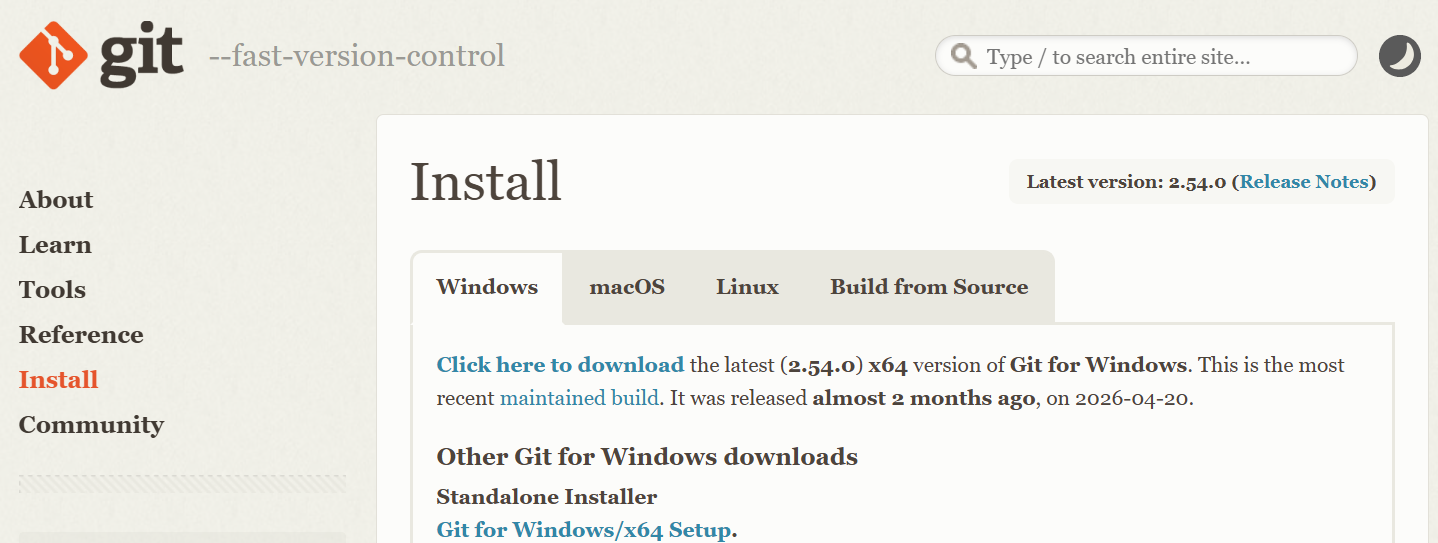
\includegraphics[width=0.5\linewidth]{21_InstallGit} \end{flushleft}

\textbf{{[}For Windows users{]}}

\begin{itemize}
\tightlist
\item
  Click on ``Windows,'' and download the standalone installer.
\item
  During the setup wizard, you can safely keep the default options
  recommended by the installer.
\end{itemize}

\textbf{{[}For Mac/macOS users{]}}

\begin{itemize}
\item
  While you can use the installer from the official website, it is
  highly recommended to install Git via Homebrew by running the
  following command in your Terminal:

\begin{verbatim}
brew install git
\end{verbatim}
\end{itemize}

\paragraph{\texorpdfstring{2.2 Create a Github
Account}{2.2 Create a Github Account }}\label{create-a-github-account}

Just as you need a Google account to access a shared Google Doc, you
need a GitHub account to access the team's cloud workspace. Once
created, share your username with your project manager so they can grant
you access to the repository.

\paragraph{\texorpdfstring{2.3 Connect RStudio to
Github}{2.3 Connect RStudio to Github }}\label{connect-rstudio-to-github}

This setup creates a direct link between the team's cloud repository and
your PC. Once completed, your RStudio environment will be fully
synchronized with GitHub and ready for using the ``Pull'' and ``Push''
buttons inside RStudio.

\textbf{Steps to connect RStudio to Github:}

\begin{enumerate}
\def\labelenumi{\alph{enumi}.}
\tightlist
\item
  Select \textbf{``New Project''} from the Project menu (top-right
  corner or via File \textgreater{} New Project) in RStudio.
\item
  Select \textbf{``Version Control''} from the project creation wizard
  window.
\end{enumerate}

\begin{flushleft}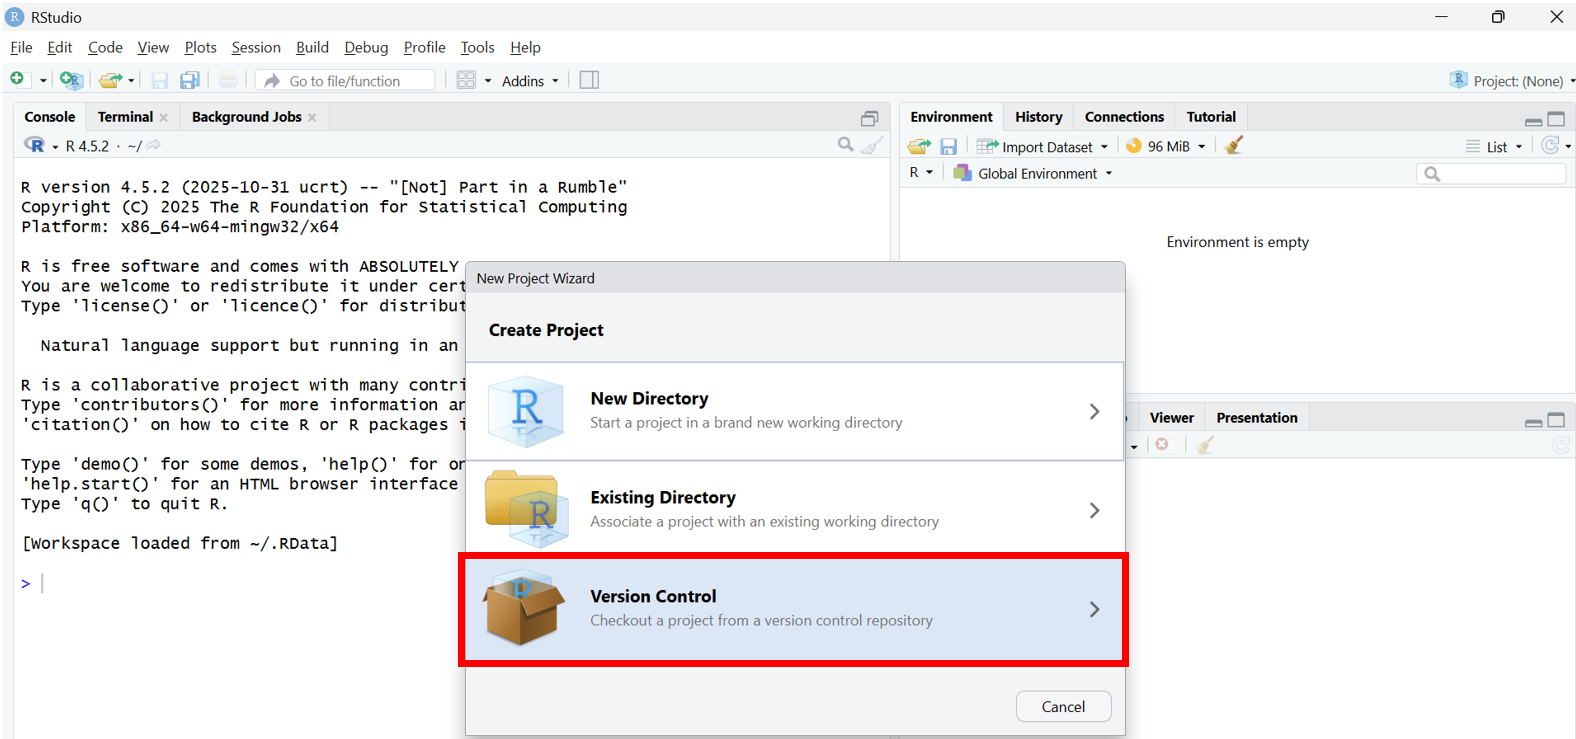
\includegraphics[width=0.7\linewidth]{23_VersionControl} \end{flushleft}

\begin{enumerate}
\def\labelenumi{\alph{enumi}.}
\setcounter{enumi}{2}
\tightlist
\item
  Select \textbf{``Git''} as your version control software.
\end{enumerate}

\begin{flushleft}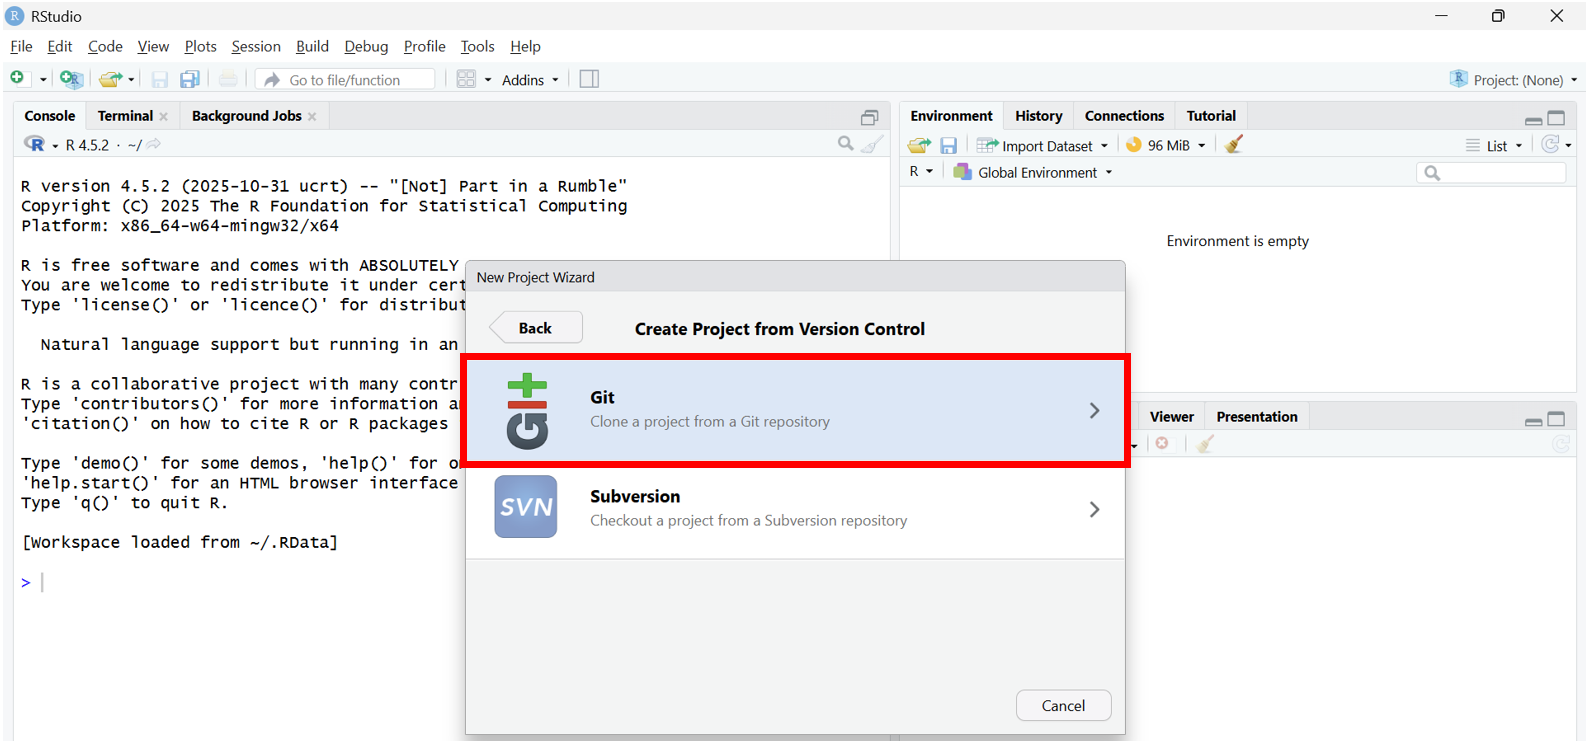
\includegraphics[width=0.7\linewidth]{23_Git} \end{flushleft}

\begin{enumerate}
\def\labelenumi{\alph{enumi}.}
\setcounter{enumi}{3}
\tightlist
\item
  Copy the Repository URL from the GitHub project page (if you do not
  have it, request the URL from your project manager).
\end{enumerate}

\begin{flushleft}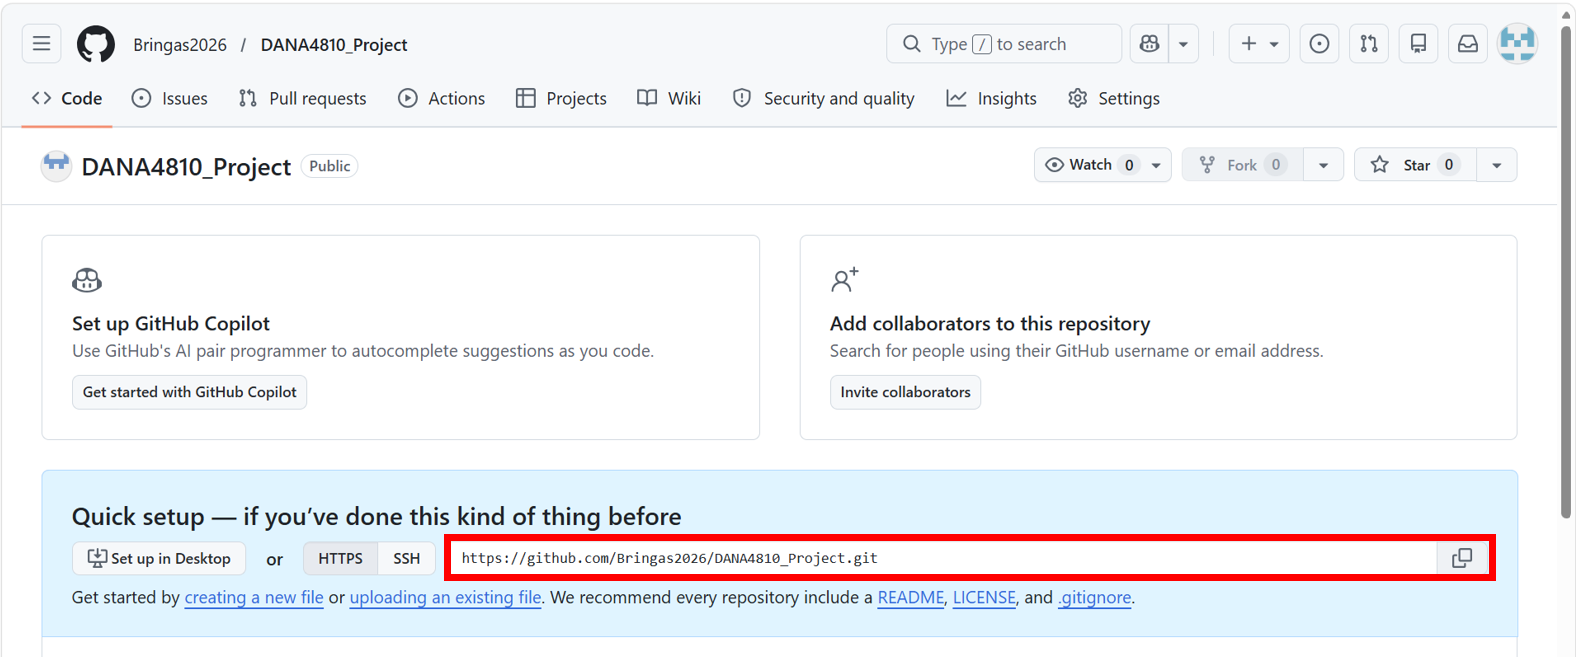
\includegraphics[width=0.7\linewidth]{23_CopyURL} \end{flushleft}

\begin{enumerate}
\def\labelenumi{\alph{enumi}.}
\setcounter{enumi}{4}
\tightlist
\item
  Paste the copied URL into the \textbf{``Repository URL''} text box
  back in RStudio. Then, click the ``Create Project'' button. The
  ``Project directory name'' field will automatically populate based on
  the repository name.
\end{enumerate}

\begin{flushleft}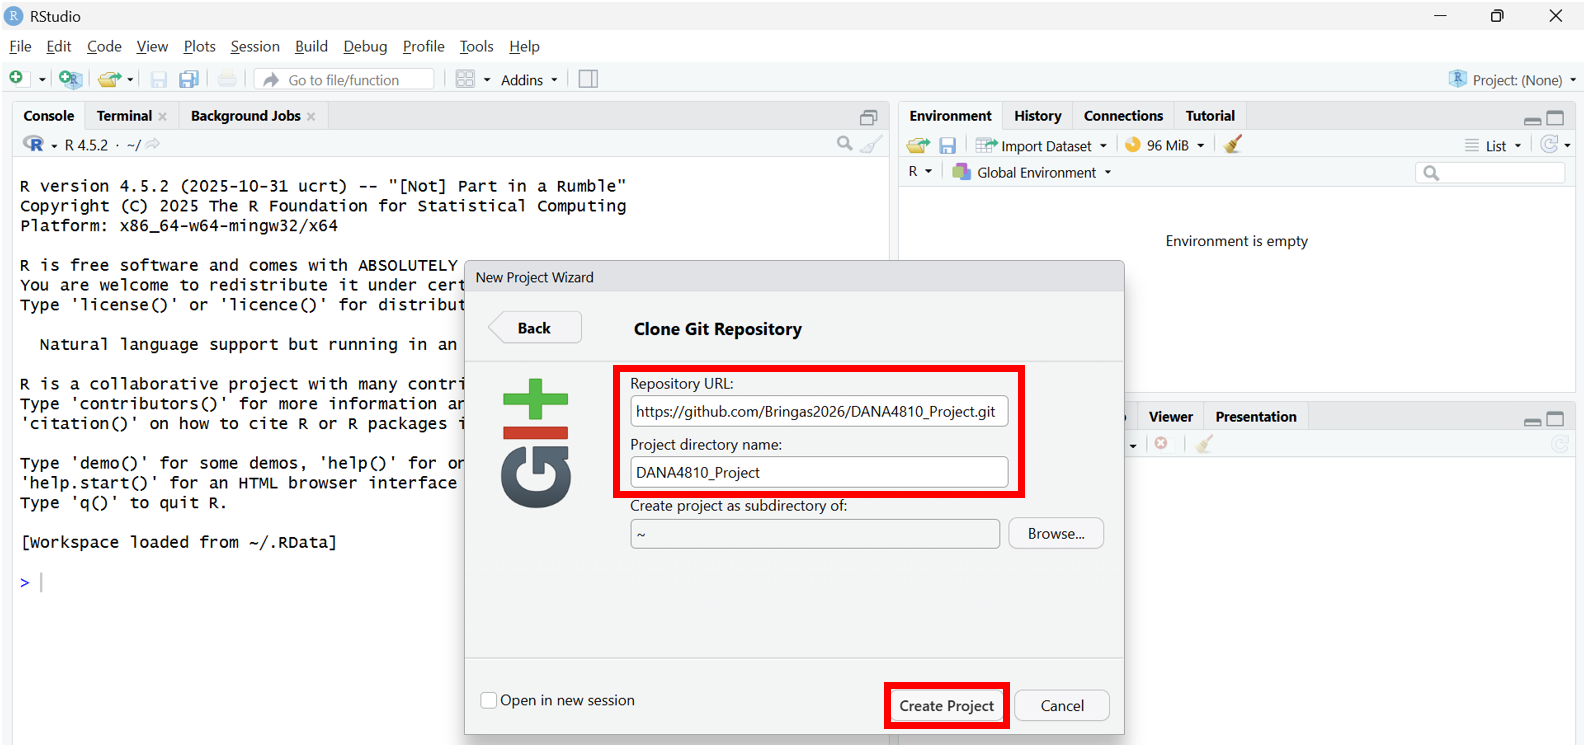
\includegraphics[width=0.7\linewidth]{23_Repo} \end{flushleft}

\begin{enumerate}
\def\labelenumi{\alph{enumi}.}
\setcounter{enumi}{5}
\tightlist
\item
  Confirm the workspace transition: RStudio will automatically refresh
  and open the new environment. Verify that the ``Git'' tab is now
  visible in your Environment pane.
\end{enumerate}

\begin{flushleft}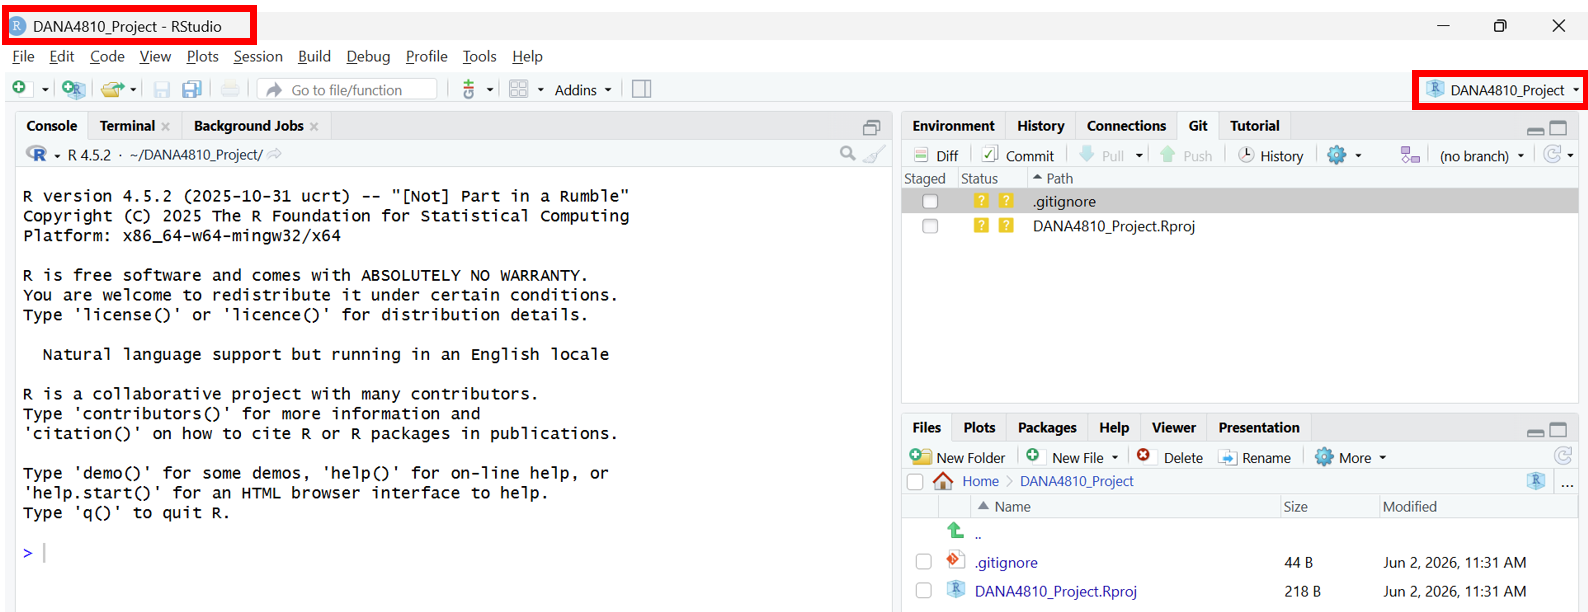
\includegraphics[width=0.7\linewidth]{23_NewProject} \end{flushleft}

\paragraph{\texorpdfstring{2.4 Setup Up Account Information \&
Credentials}{2.4 Setup Up Account Information \& Credentials }}\label{setup-up-account-information-credentials}

To make sure that each team member's name shows up in Github after
pushing, which is quite important to track update history: who made this
change, RStudio needs to be linked to appropriate Github account. ✅
Make sure to use the exact same email address you used to create your
Github account. ✅ This will be reflected only your future updates. Past
updates cannot be cahnged (although your updates themselves should be
safely pushed.)

How to do that:

\begin{enumerate}
\def\labelenumi{\arabic{enumi}.}
\tightlist
\item
  Set your Github Username
\end{enumerate}

\begin{verbatim}
git config --global user.name "Your GitHub Username"
\end{verbatim}

\begin{enumerate}
\def\labelenumi{\arabic{enumi}.}
\setcounter{enumi}{1}
\tightlist
\item
  Set your Github Email Address
\end{enumerate}

\begin{verbatim}
git config --global user.email "Your GitHub Email Address"
\end{verbatim}

\begin{center}\rule{0.5\linewidth}{0.5pt}\end{center}

\subsubsection{3. Basic Operation for Daily
Use}\label{basic-operation-for-daily-use}

\textbf{As a Golden Rule of GitHub, always follow this order every
single day}

\begin{quote}
{[}PULL{]} → {[}EDIT{]} → {[}STAGE{]} → {[}COMMIT{]} → {[}PUSH{]}
\end{quote}

✅ Skip ``Pull'' at the start and you risk creating conflicts with your
teammates' work.

\begin{center}\rule{0.5\linewidth}{0.5pt}\end{center}

\textbf{As a Key Concept, there are three Git Environments: Local,
Staging, and GitHub} To collaborate effectively, it is essential to
understand that Git manages your work across three separate stages,
which is a major shift from the automatic, single-layer syncing of
Google Docs:

\begin{enumerate}
\def\labelenumi{\arabic{enumi}.}
\item
  \textbf{Local Environment}: Your local machine where you open RStudio
  and edit code. Saving files here affects your local disk only,
  ensuring a safe sandbox where you can test or break code without
  impacting others.
\item
  \textbf{Staging Area}: A critical intermediary stage. When you create
  a ``Commit,'' the files currently in the Staging Area are recorded
  directly into your Local Repository (your PC's history log). It is
  crucial to note that committing does NOT send your changes to GitHub
  yet; your work remains strictly on your local machine until you
  ``Push.''
\item
  \textbf{GitHub (Remote Repository)}: The shared cloud infrastructure.
  Once your staged files are committed, hitting ``Push'' transfers those
  snapshots to GitHub, updating the team's official master copy.
\end{enumerate}

Note: The Purpose of Staging The Staging Area acts as a filter. Instead
of throwing all ongoing modifications into the cloud at once, it allows
you to selectively package and comment on your changes step-by-step.
This structural control is what gives Git its superior version tracking
capabilities compared to traditional word processors.

\paragraph{3.1 Open RStudio}\label{open-rstudio}

Launch the RStudio application on your local machine to begin your
workspace.

\begin{flushleft}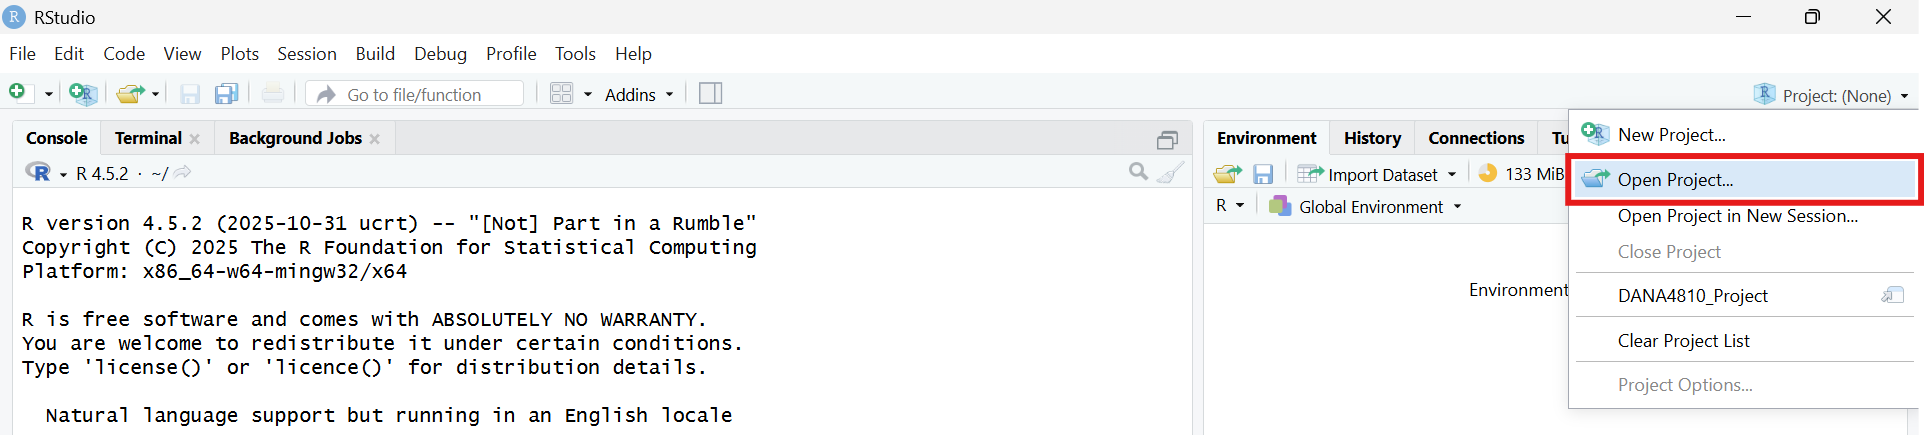
\includegraphics[width=0.8\linewidth]{31_OpenProject} \end{flushleft}

\paragraph{3.2 Select a Project}\label{select-a-project}

Open your team's designated collaborative project by selecting the
corresponding .Rproj file from the project menu.

\begin{flushleft}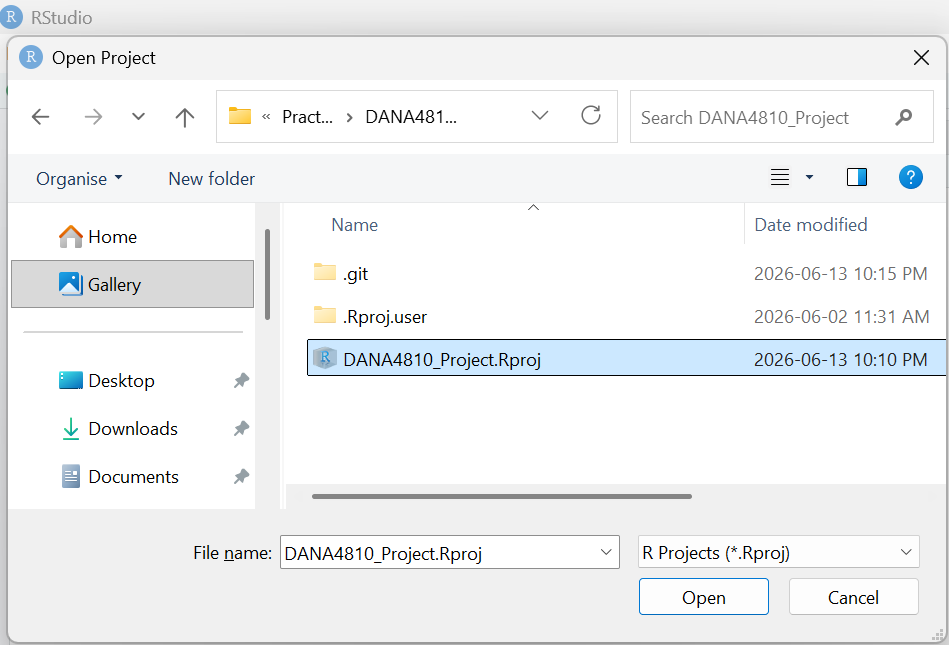
\includegraphics[width=0.3\linewidth]{32_SelectProject} \end{flushleft}

\paragraph{3.3 Pull the latest files from GitHub
{[}PULL{]}}\label{pull-the-latest-files-from-github-pull}

Navigate to the Git tab and click the \textbf{``Pull''} button to
synchronize your local environment with the latest changes made by your
team on GitHub. Always do this before you start writing any code to
prevent future conflicts.

\begin{flushleft}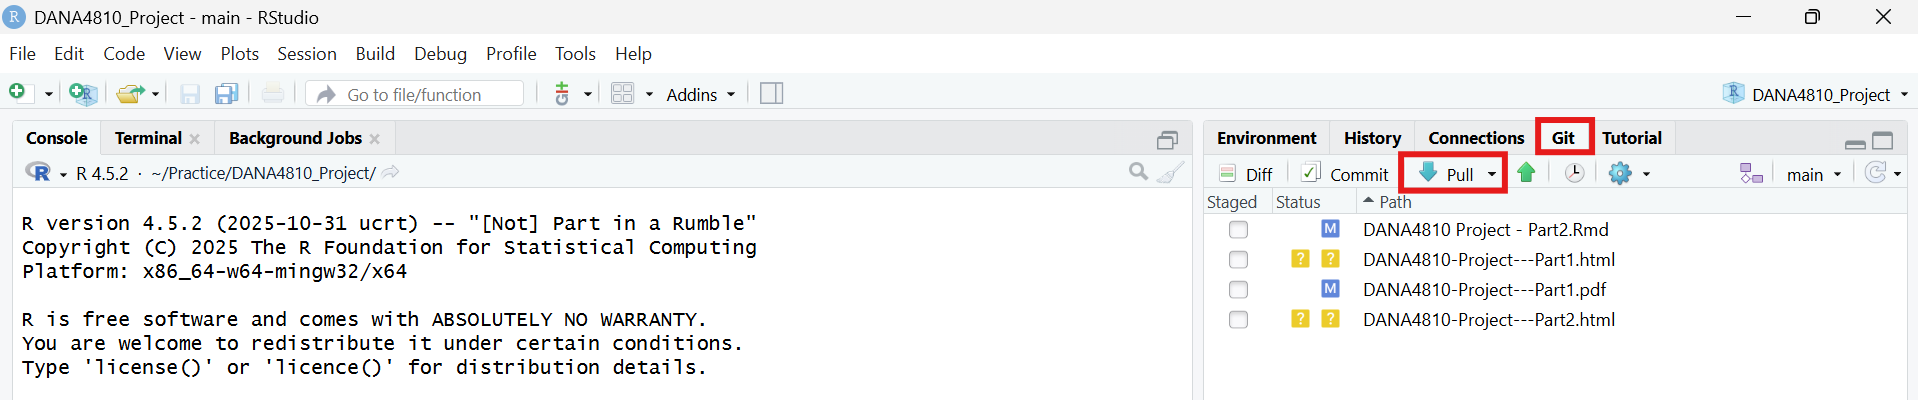
\includegraphics[width=0.8\linewidth]{33_Pull} \end{flushleft}

\paragraph{3.4 Modify and Save files locally
{[}EDIT{]}}\label{modify-and-save-files-locally-edit}

After completing your edits in files, save your progress locally by
pressing Ctrl+S (Windows) or Cmd+S (Mac).

\begin{flushleft}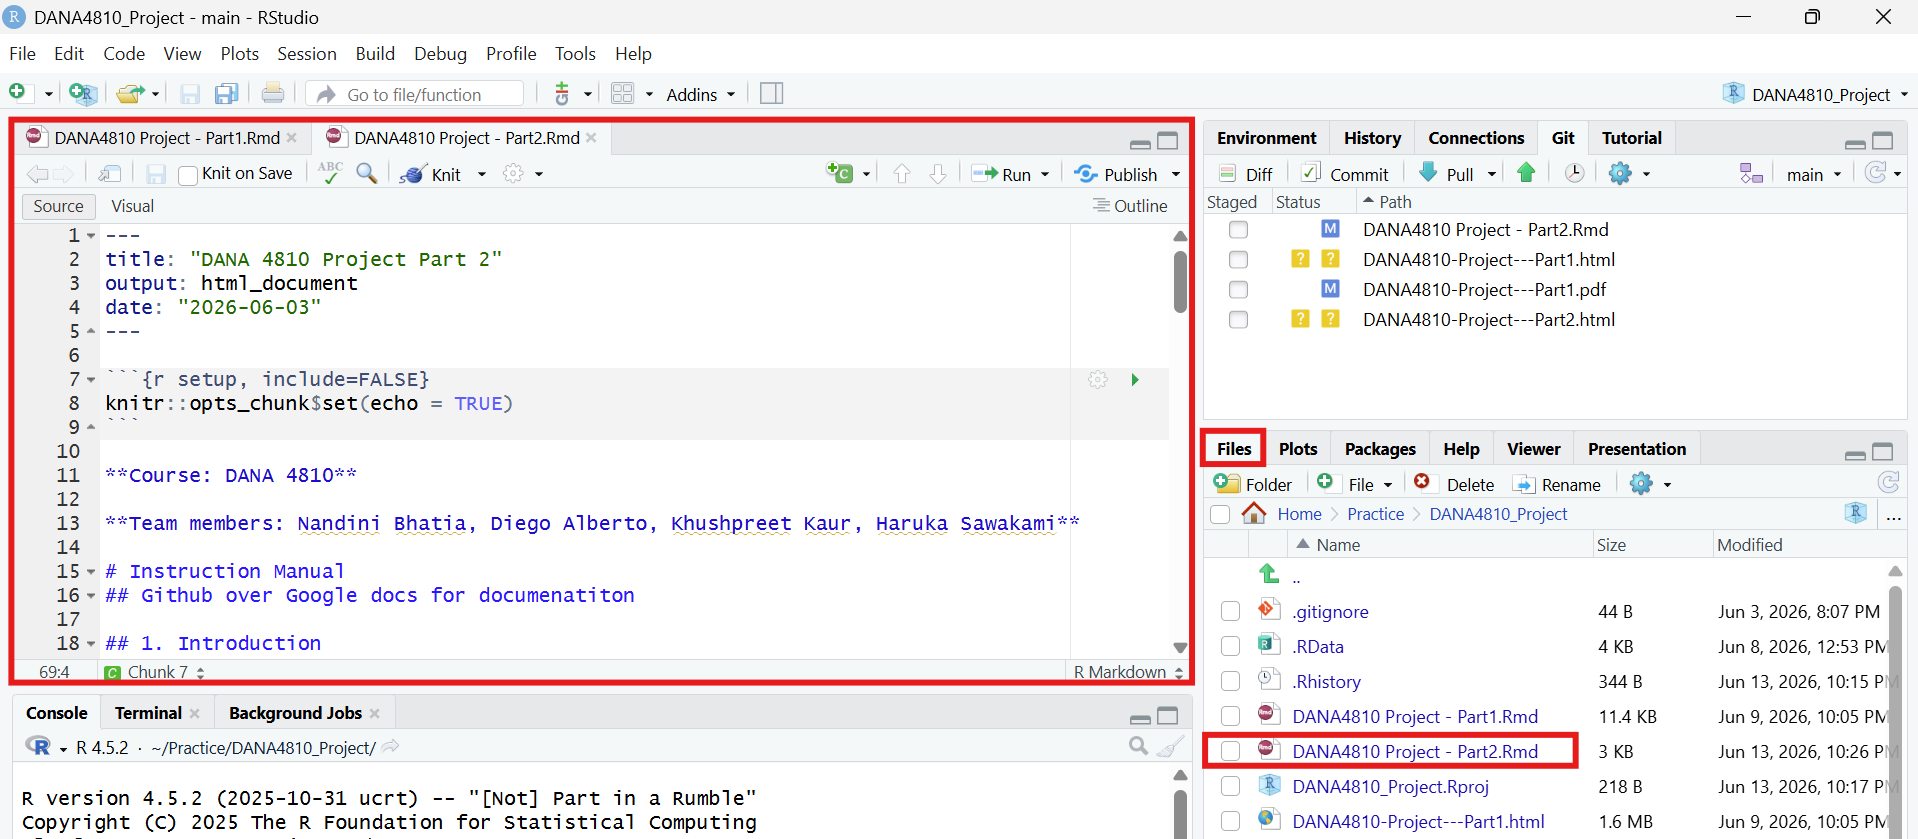
\includegraphics[width=0.8\linewidth]{34_Modify&Save} \end{flushleft}

\paragraph{3.5 Commit your changes with a clear comment
{[}STAGE\&COMMIT{]}}\label{commit-your-changes-with-a-clear-comment-stagecommit}

Check the \textbf{``Staged''} box next to the modified files in the Git
tab, click \textbf{``Commit''}, and log a concise, descriptive
\textbf{Commit message} explaining your updates. Note: When making your
first commit, RStudio may prompt you to enter your username and email
address. If this occurs, please follow the steps in ``2.4 Setup Up
Account Information \& Credentials'' to complete the configuration.

\begin{flushleft}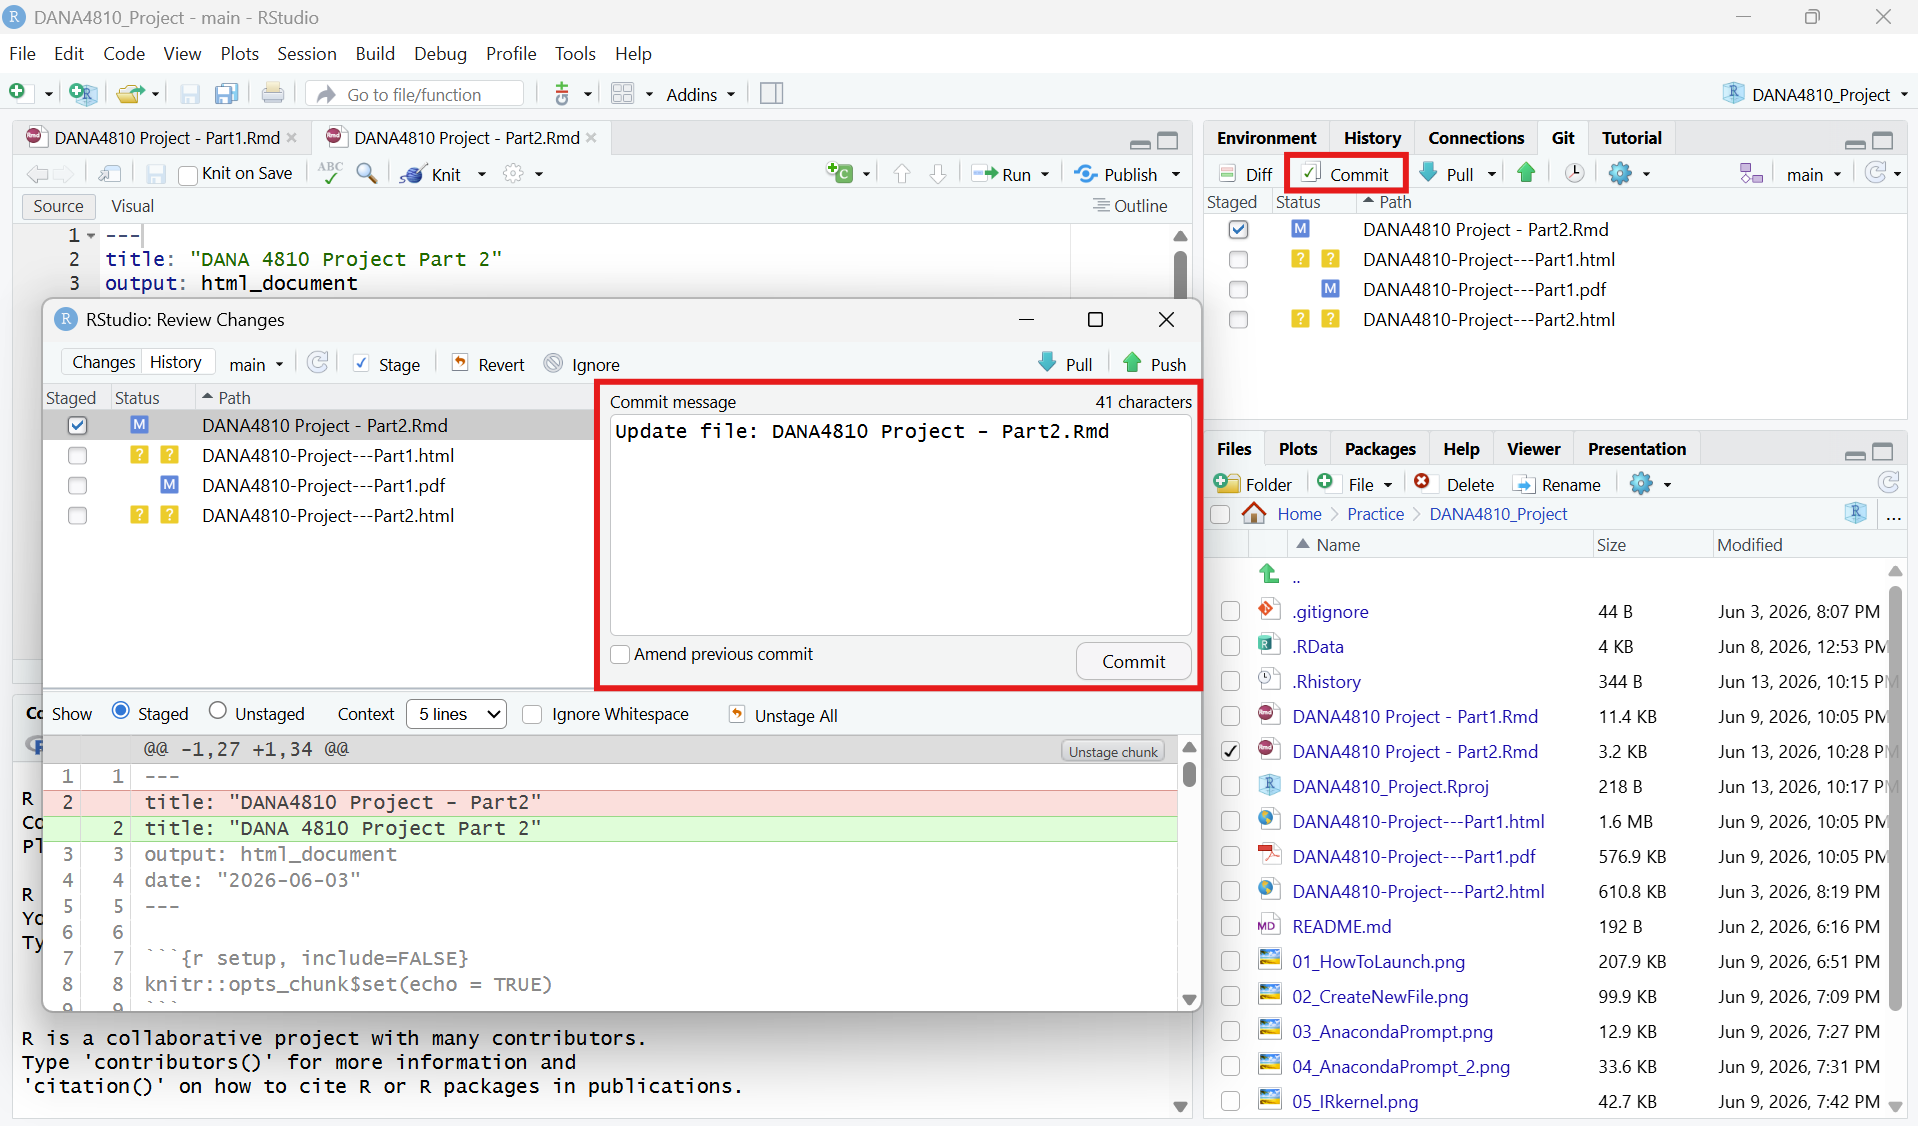
\includegraphics[width=0.8\linewidth]{35_Commit} \end{flushleft}

\paragraph{3.6 Push your commits to Github
{[}PUSH{]}}\label{push-your-commits-to-github-push}

Click the \textbf{``Push''} button to upload your recorded local
snapshots to the shared GitHub repository, making your contributions
visible to the entire team. You may find the \textbf{``Push''} button on
the previous Commit screen named ``Review Changes''. Both works in the
same way.

\begin{flushleft}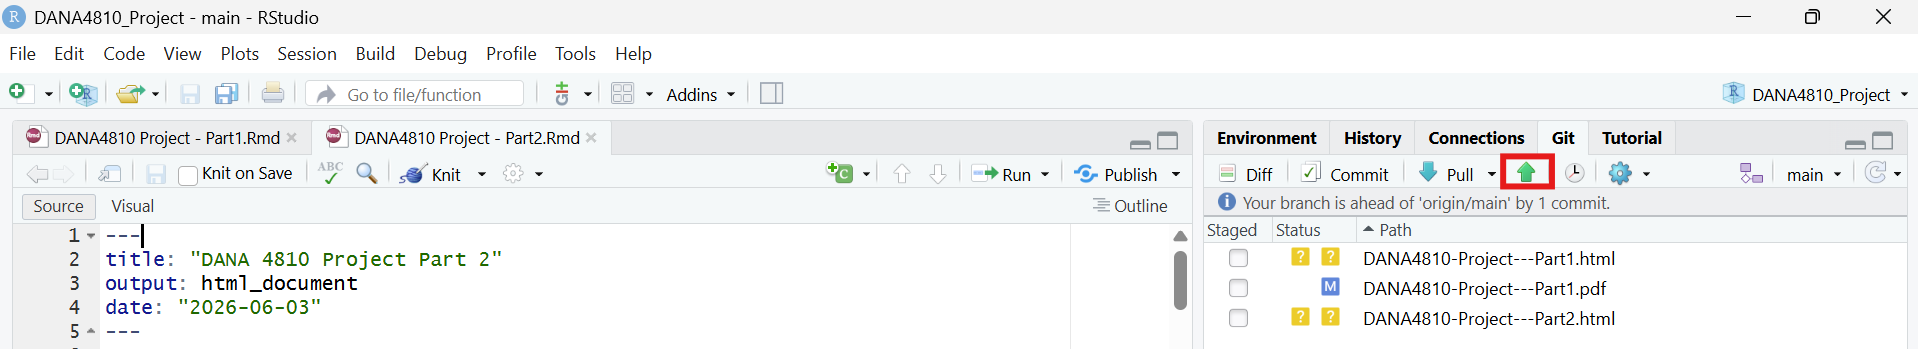
\includegraphics[width=0.8\linewidth]{36_Push} \end{flushleft}

\begin{center}\rule{0.5\linewidth}{0.5pt}\end{center}

\subsubsection{4. Version Control}\label{version-control}

Version Control is a good practice that manages changes files over time.
It acts like digital audit trails, allowing you to see exactly who made
what changes, when and allows to revert to previous states if mistake
occurs. While Google Docs automatically saves your work with every
single keystroke, GitHub records a ``version'' (snapshot) only when a
user intentionally creates a ``Commit.''

\paragraph{4.1 How to make a version}\label{how-to-make-a-version}

As a brief recap from Section 3, your changes are only safely logged as
a official ``version'' once you complete both the Commit and Push
operations. Remember, clicking ``Commit'' records the snapshot to your
local history, and clicking ``Push'' uploads it to GitHub to make it
permanent for the team.

\textbf{Steps to create a commit in RStudio:}

\begin{enumerate}
\def\labelenumi{\alph{enumi}.}
\tightlist
\item
  Make and save your changes to the files as normal.
\item
  In RStudio, open the Git tab (top-right panel).
\item
  Check the box next to each file you changed --- this stages the file.
\item
  Click Commit.
\item
  In the box that appears, type a short commit message describing what
  you did.
\item
  Click Commit to confirm.
\end{enumerate}

✅ A good commit message answers the question: \emph{``What did this
change do?''} --- not just \emph{``I changed something.''}

\paragraph{4.2 How to check a history and
differences}\label{how-to-check-a-history-and-differences}

You can review your project's commit history either directly inside
\textbf{RStudio} or via the \textbf{GitHub Web interface}, depending on
your needs. Use the RStudio Git History for a quick check on your local
incremental changes and code differences (Diff) while working. For a
comprehensive, visual overview of all team activities, timeline
tracking, and repository-wide updates, reviewing the history on the
GitHub Web interface is highly recommended.

\textbf{In RStudio:}

\begin{itemize}
\tightlist
\item
  Click the \textbf{clock icon} in the Git tab to open the commit
  history for your project.
\end{itemize}

\begin{flushleft}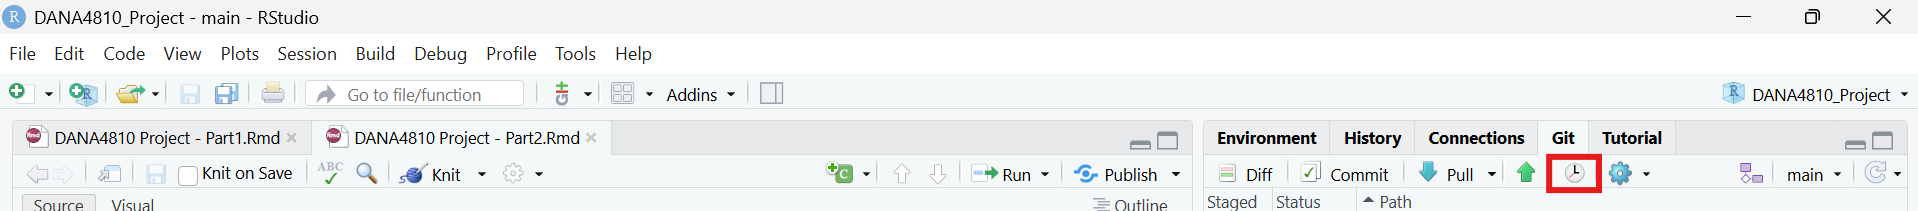
\includegraphics[width=0.8\linewidth]{42_History} \end{flushleft}

\begin{itemize}
\item
  Each row shows the commit message, the author's name, and the date.
\item
  Click any commit to see a \textbf{diff} (a colour-coded comparison):

  \begin{itemize}
  \tightlist
  \item
    \textbf{Green lines} = content that was added
  \item
    \textbf{Red lines} = content that was removed
  \end{itemize}
\end{itemize}

\begin{flushleft}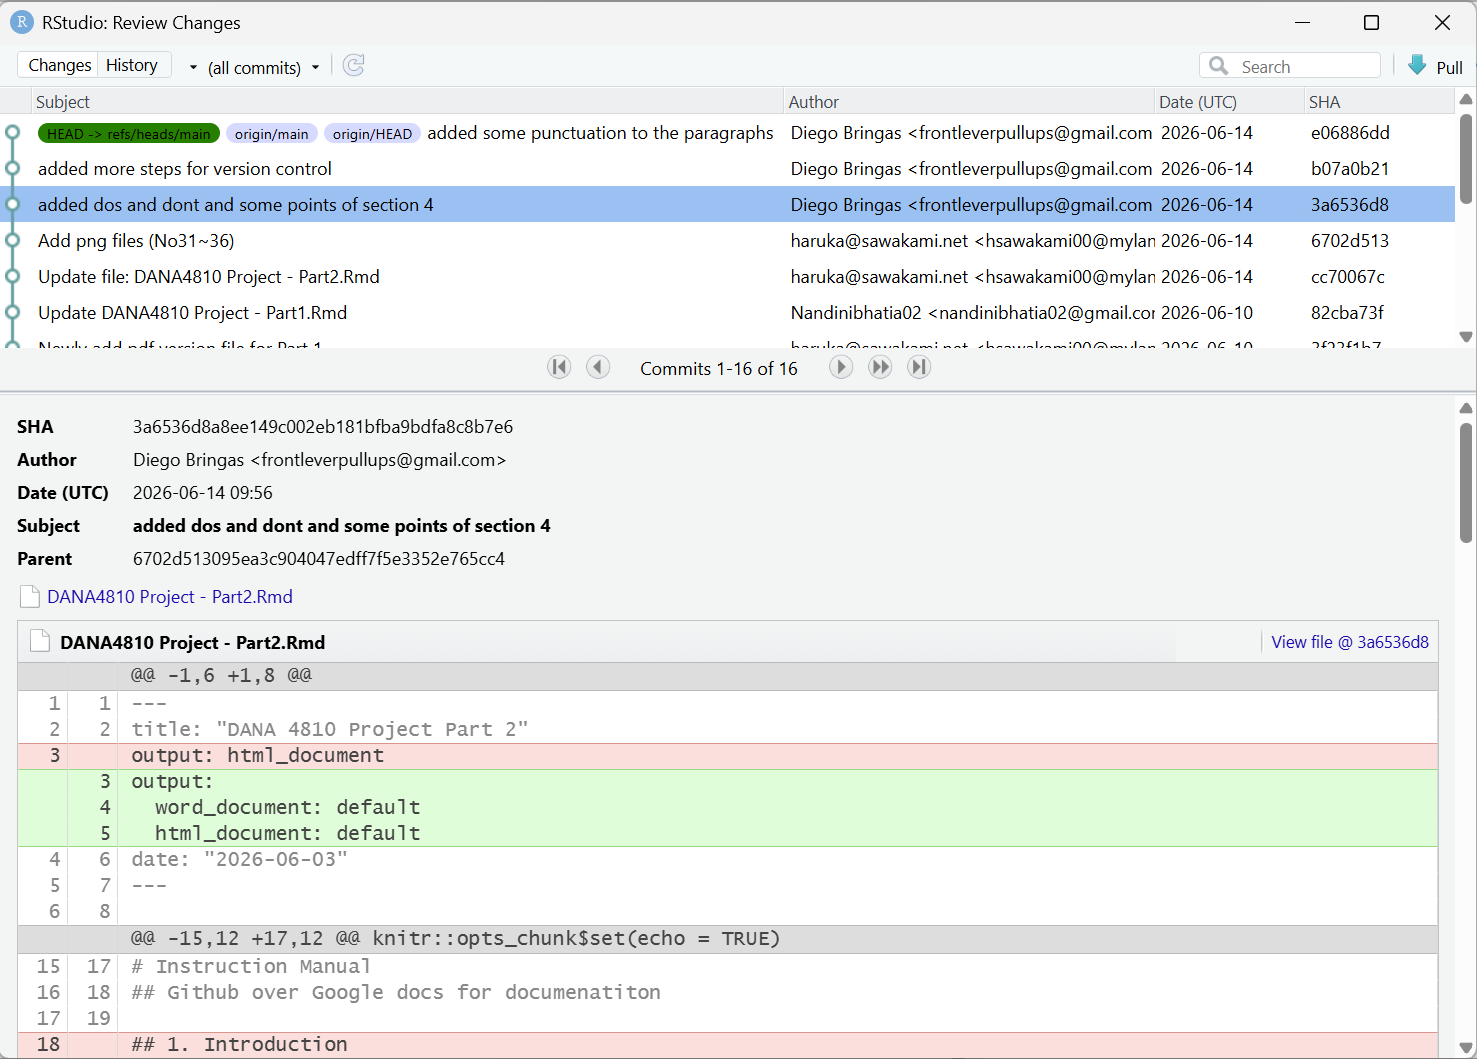
\includegraphics[width=0.7\linewidth]{42_Diff} \end{flushleft}

\textbf{On GitHub.com:}

\begin{enumerate}
\def\labelenumi{\arabic{enumi}.}
\tightlist
\item
  Open your repository on GitHub.
\item
  Click \textbf{Commits} (near the top of the file list) to see the full
  history.
\end{enumerate}

\begin{flushleft}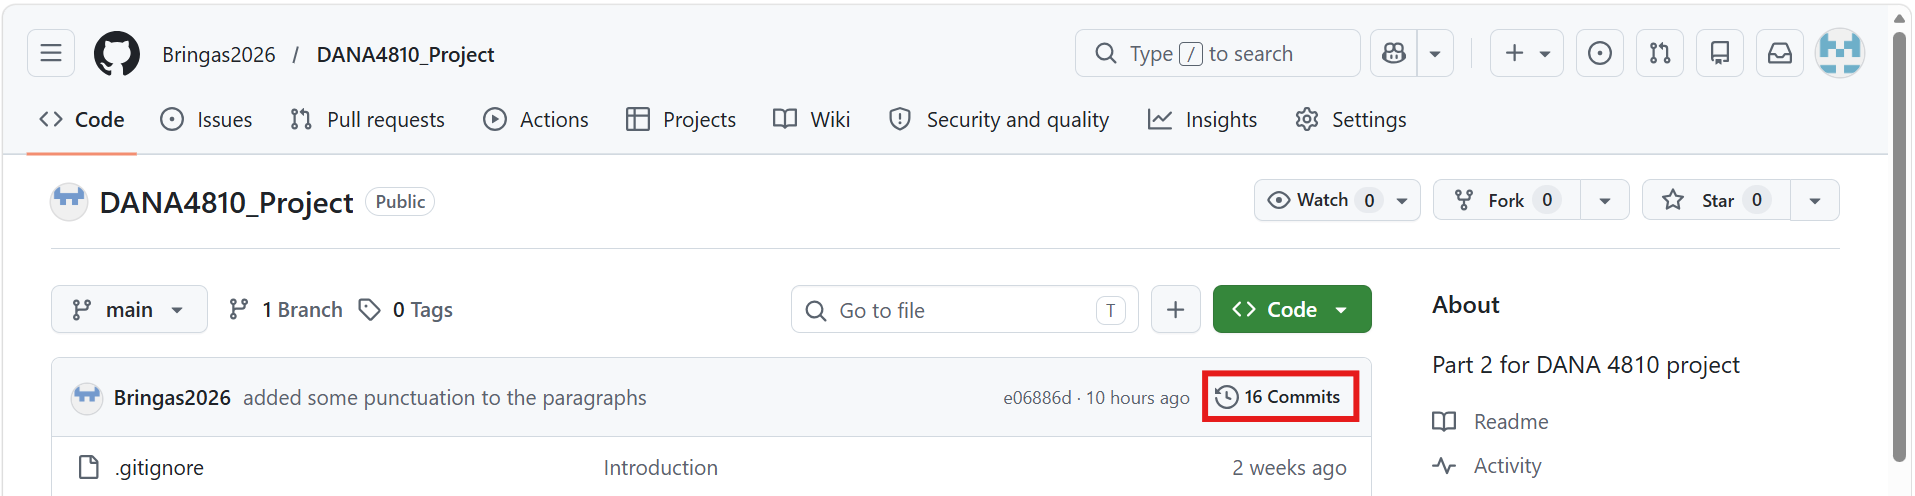
\includegraphics[width=0.7\linewidth]{42_History(GitHub)} \end{flushleft}

\begin{enumerate}
\def\labelenumi{\arabic{enumi}.}
\setcounter{enumi}{2}
\tightlist
\item
  Click any commit to see exactly which lines were added or removed in
  every file.
\item
  To see who wrote each specific line of a file, open the file and click
  \textbf{Blame}. GitHub will annotate every line with the author and
  the date it was last changed.
\end{enumerate}

\begin{flushleft}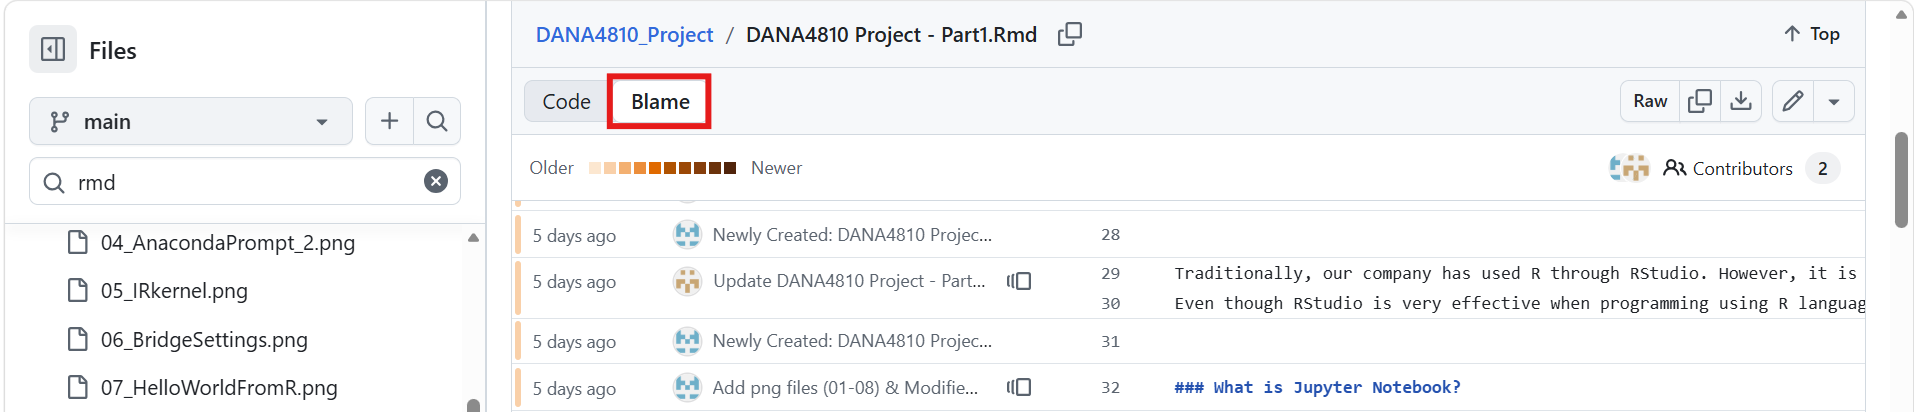
\includegraphics[width=0.8\linewidth]{42_Diff(GitHub)} \end{flushleft}

\paragraph{4.3 How to restore from a Local Changes (Before
Commit)}\label{how-to-restore-from-a-local-changes-before-commit}

If you have edited a file but have not yet committed, you can discard
your local changes and return the file to the last committed version.

\textbf{In RStudio:}

\begin{enumerate}
\def\labelenumi{\arabic{enumi}.}
\tightlist
\item
  In the \textbf{Git} tab, right-click the file you want to restore.
\item
  Select \textbf{Revert\ldots{}} and confirm.
\end{enumerate}

\begin{flushleft}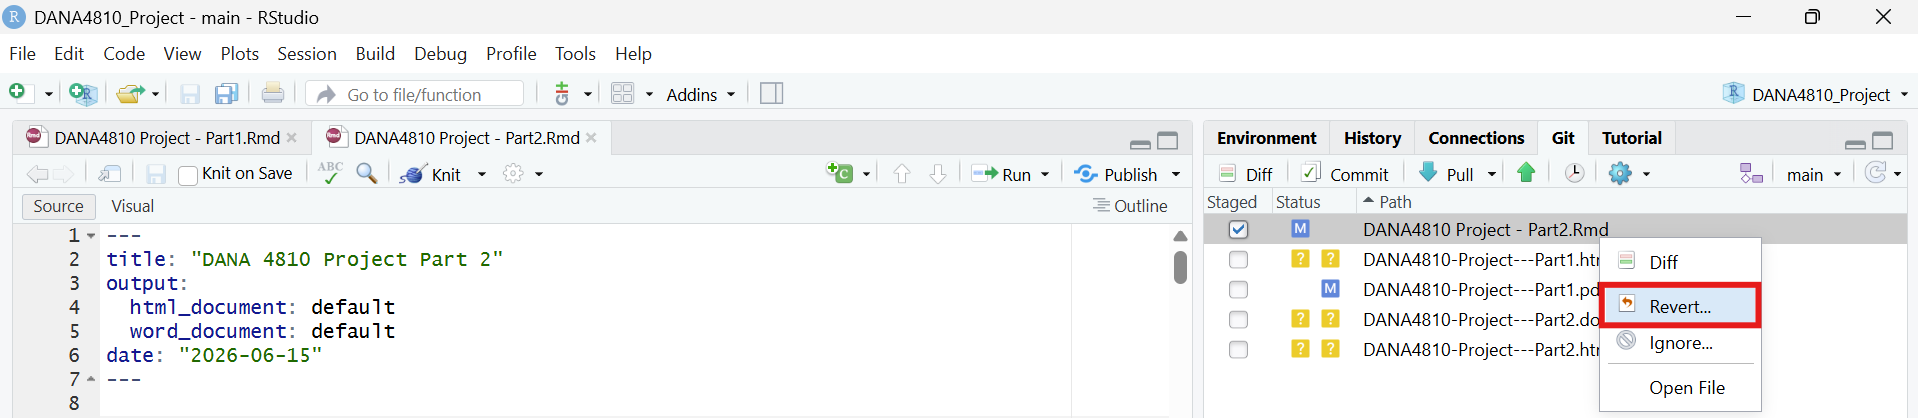
\includegraphics[width=0.8\linewidth]{43_Revert} \end{flushleft}

\textbf{In the terminal:}

\begin{verbatim}
git checkout -- filename.Rmd
\end{verbatim}

\paragraph{4.4 How to restore from a Past Commit
(Local)}\label{how-to-restore-from-a-past-commit-local}

If you have already committed a change but want to go back to an earlier
version of a specific file, you can restore it using the commit's unique
ID (called a \textbf{hash}).

\textbf{Steps:}

\begin{enumerate}
\def\labelenumi{\arabic{enumi}.}
\tightlist
\item
  Open the \textbf{Git} tab in RStudio and click the \textbf{clock icon}
  to view history.
\end{enumerate}

\begin{flushleft}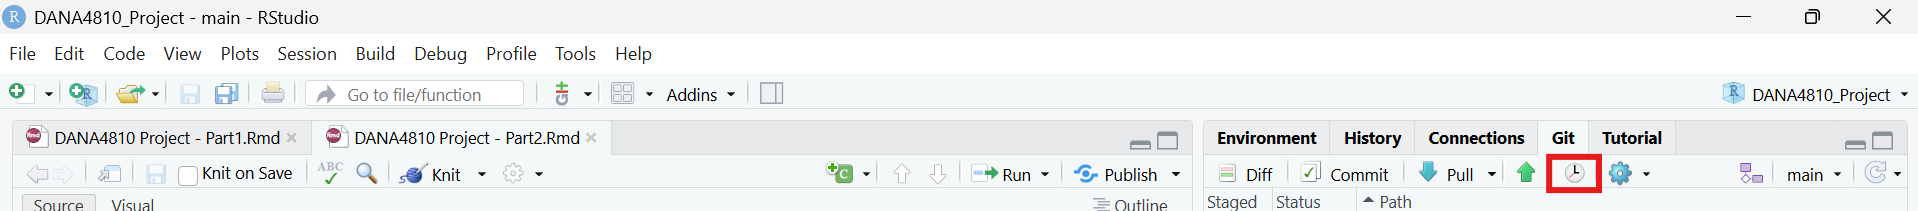
\includegraphics[width=0.8\linewidth]{42_History} \end{flushleft}

\begin{enumerate}
\def\labelenumi{\arabic{enumi}.}
\setcounter{enumi}{1}
\tightlist
\item
  Find the commit you want to restore and copy its short hash / SHA
  (e.g., \texttt{3a6536d8}).
\end{enumerate}

\begin{flushleft}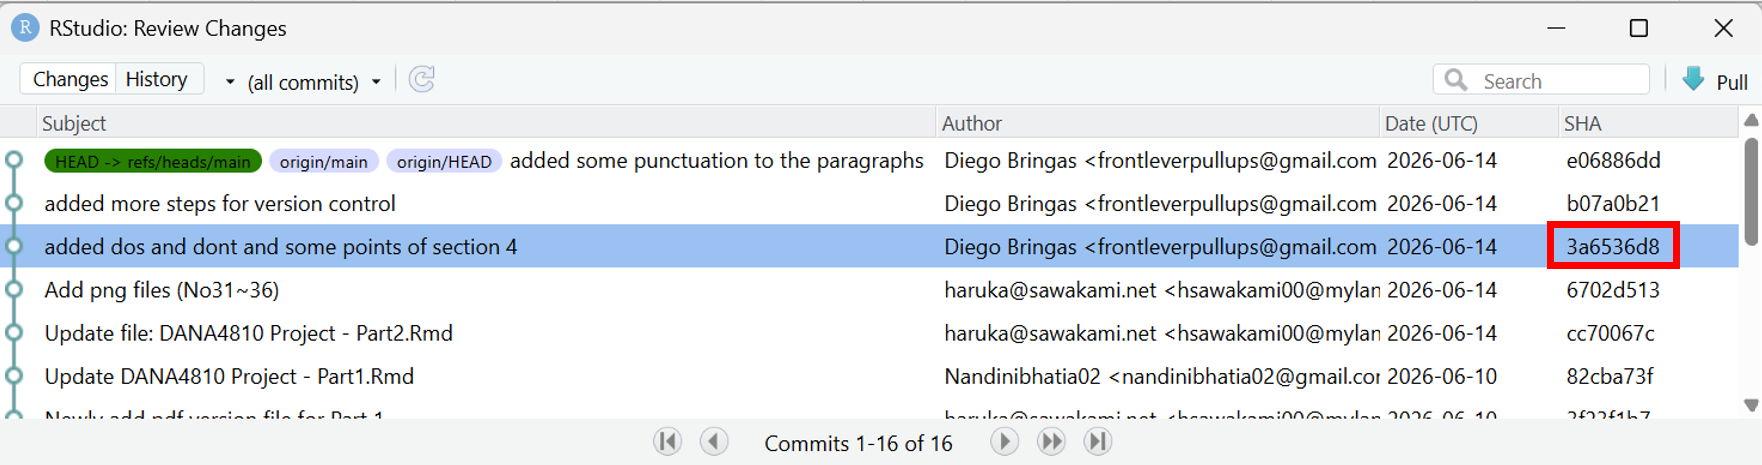
\includegraphics[width=0.8\linewidth]{44_Hash} \end{flushleft}

\begin{enumerate}
\def\labelenumi{\arabic{enumi}.}
\setcounter{enumi}{2}
\tightlist
\item
  In the RStudio terminal, run:
\end{enumerate}

\begin{verbatim}
git checkout 3a6536d8 -- filename.Rmd
\end{verbatim}

\begin{enumerate}
\def\labelenumi{\arabic{enumi}.}
\setcounter{enumi}{3}
\tightlist
\item
  Stage it and commit again:
\end{enumerate}

\begin{verbatim}
git add filename.Rmd
git commit -m "Restore filename.Rmd to version from [date]"
\end{verbatim}

\begin{enumerate}
\def\labelenumi{\arabic{enumi}.}
\setcounter{enumi}{4}
\tightlist
\item
  Push the commit so the rest of the team also sees the restored version
  --- either run \texttt{git\ push}, or simply click the
  \textbf{``Push''} button in RStudio as in Section 3.6.
\end{enumerate}

\begin{flushleft}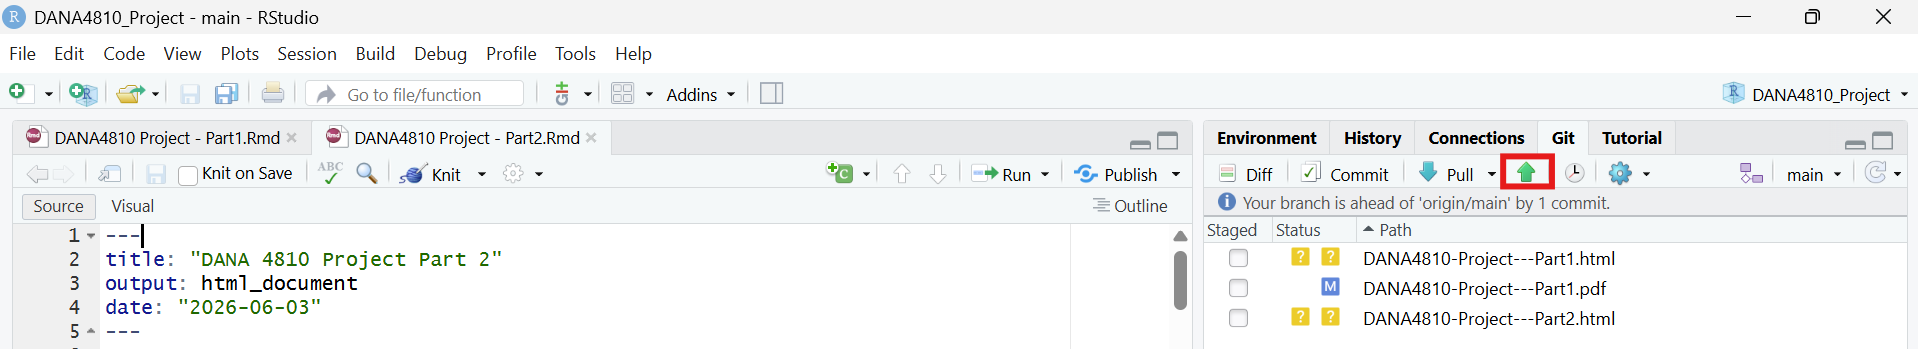
\includegraphics[width=0.8\linewidth]{36_Push} \end{flushleft}

\paragraph{4.5 How to restore from a
Github}\label{how-to-restore-from-a-github}

\textbf{- Pulling the latest version from GitHub (safest):}

\begin{verbatim}
git pull origin main
\end{verbatim}

This will automatically download any commits made on Github and merge
them with your files.

\paragraph{4.6 How to communicate with team
members}\label{how-to-communicate-with-team-members}

Good communication is what keeps a team from stepping on each other's
work. GitHub gives you several built-in tools for this:

\textbf{Commit messages as communication:}

Every commit message is visible to the whole team in the history.
Writing clear messages means your teammates always know what you were
working on without having to ask.

\begin{verbatim}
# Examples of helpful commit messages:
"Add Section 3 daily workflow steps"
"Fix merge conflict in introduction"
"Update Do's and Don'ts table with new examples"
\end{verbatim}

\textbf{GitHub Issues:}

Issues are like a built-in task board inside your repository. You can
use them to:

\begin{itemize}
\tightlist
\item
  Report a problem (e.g., ``Section 4.2 screenshot is missing'')
\item
  Assign tasks to specific team members
\item
  Track progress --- close the Issue when the task is done
\end{itemize}

\textbf{Steps to create an Issue:}

\begin{enumerate}
\def\labelenumi{\arabic{enumi}.}
\tightlist
\item
  Go to your repository on GitHub.
\item
  Click the \textbf{Issues} tab.
\item
  Click \textbf{New Issue}, describe the task or problem, and click
  \textbf{Submit}.
\end{enumerate}

\begin{flushleft}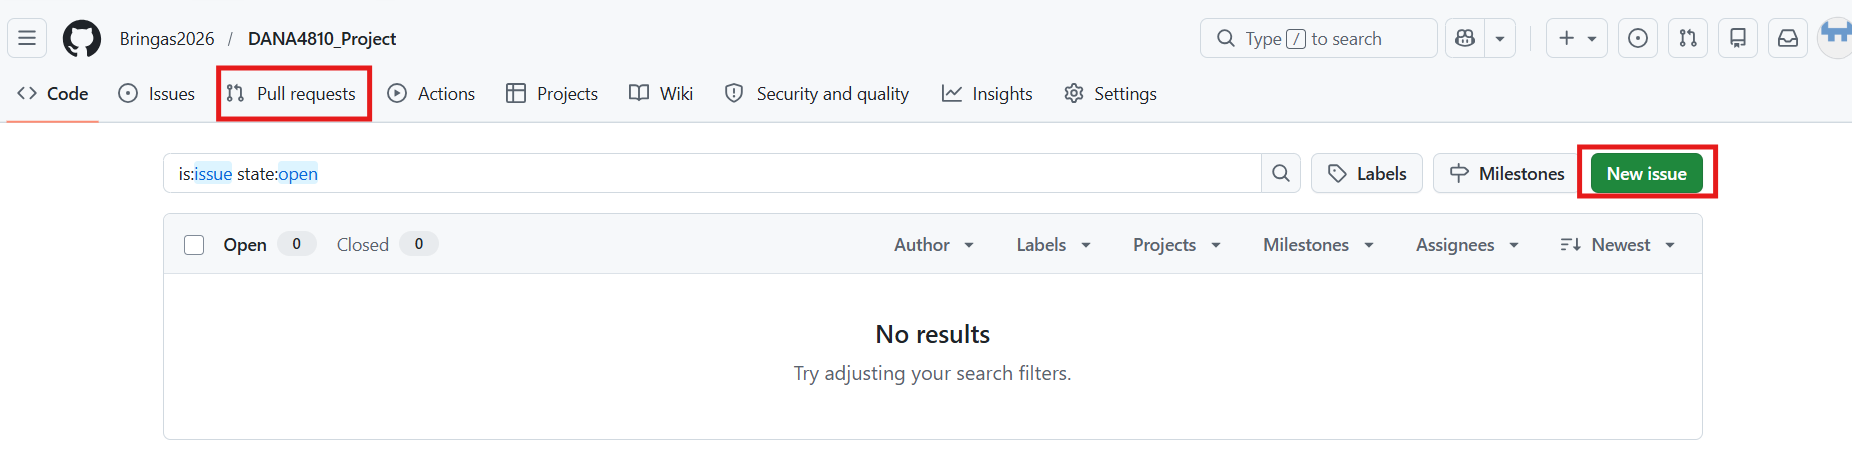
\includegraphics[width=0.8\linewidth]{53_Issues} \end{flushleft}

\textbf{Pull Request comments:}

When a teammate reviews your work before it gets merged into
\texttt{main} (see Section 5.1), they leave their feedback directly on
the Pull Request as comments. This keeps the whole discussion about a
change attached to the exact lines being discussed, instead of getting
scattered across email or chat.

\begin{flushleft}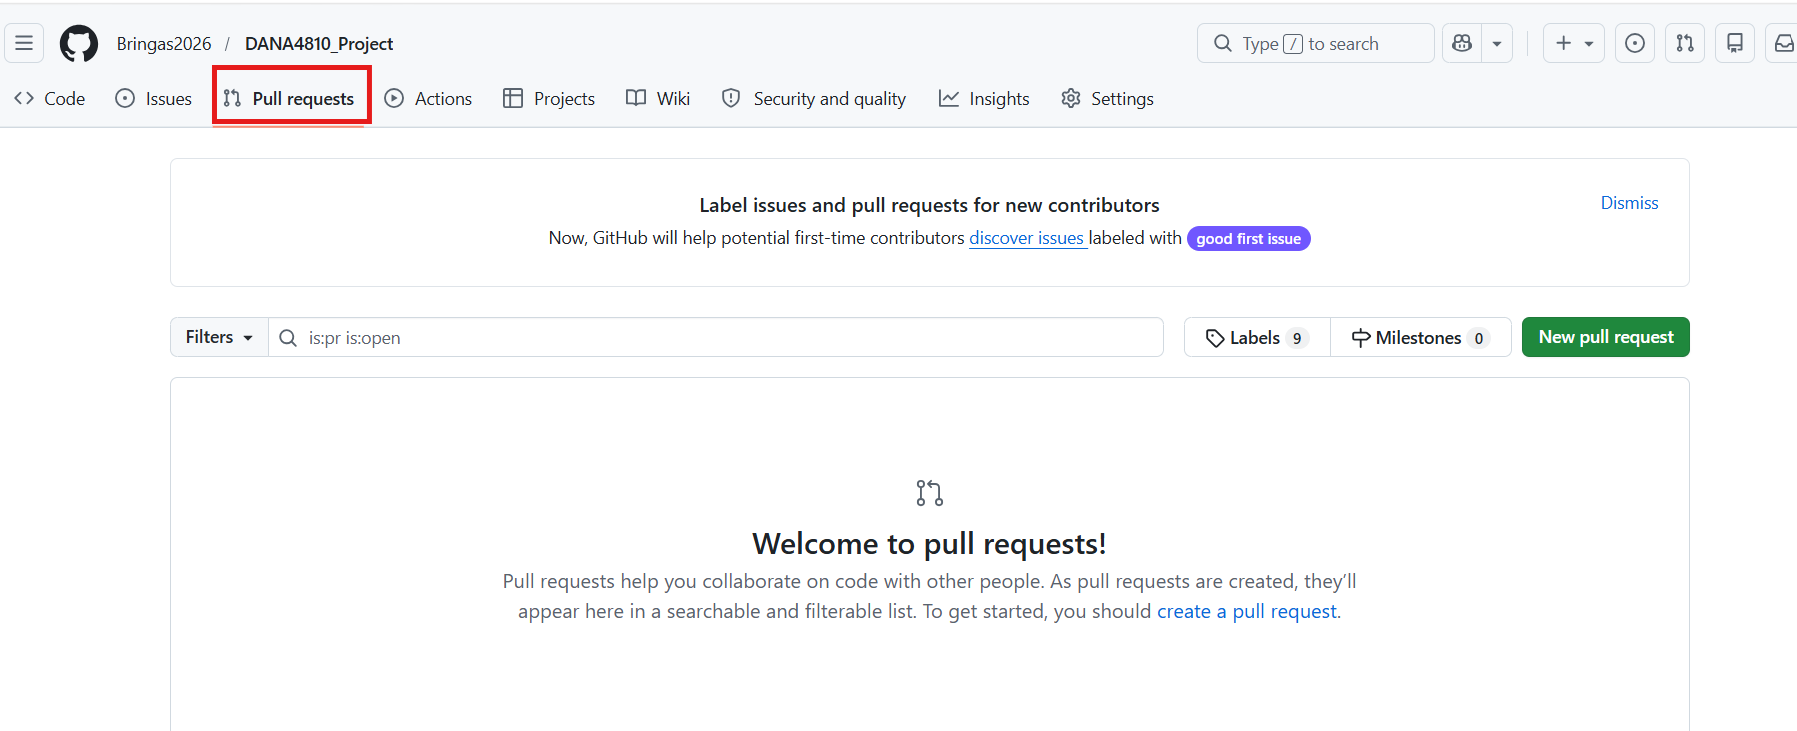
\includegraphics[width=0.8\linewidth]{54_PullRequest} \end{flushleft}

\paragraph{4.7 Understanding Branches}\label{understanding-branches}

A \textbf{branch} is an independent copy of the project where you can
work freely without affecting the \texttt{main} version that everyone
shares. Think of it like making a photocopy of a document to draft edits
on --- you only update the original once you are happy with your
changes.

\textbf{Why branches matter for teams:}

\begin{itemize}
\tightlist
\item
  Team members can work on different features at the same time without
  interfering with each other
\item
  The \texttt{main} branch always stays clean and working
\item
  If something breaks on your branch, it does not affect anyone else
\end{itemize}

\textbf{How to create a branch in RStudio:}

\begin{enumerate}
\def\labelenumi{\arabic{enumi}.}
\tightlist
\item
  In the Git tab, click the \textbf{branch icon} (purple icon near the
  top right of the Git pane).
\end{enumerate}

\begin{flushleft}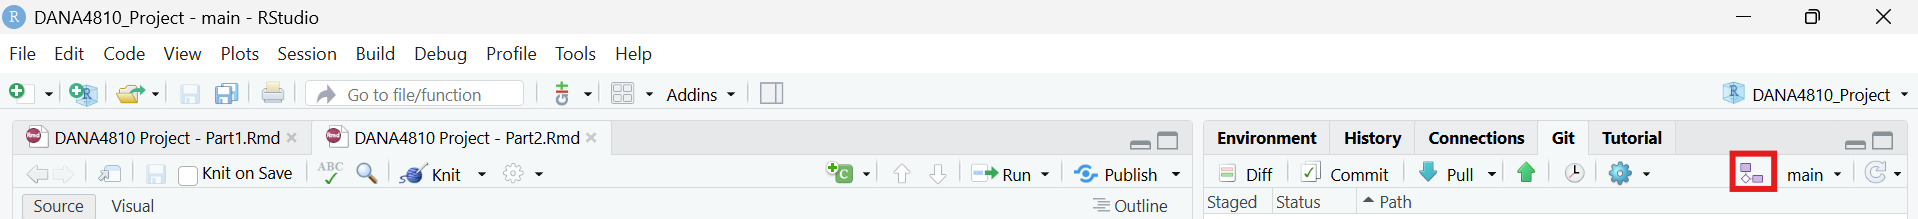
\includegraphics[width=0.8\linewidth]{47_Branch} \end{flushleft}

\begin{enumerate}
\def\labelenumi{\arabic{enumi}.}
\setcounter{enumi}{1}
\tightlist
\item
  Type a descriptive name for your branch (e.g.,
  \texttt{feature/add-section-5} or \texttt{fix/typo-introduction}).
\item
  Click \textbf{Create}. RStudio will automatically switch you to that
  branch
\end{enumerate}

\begin{flushleft}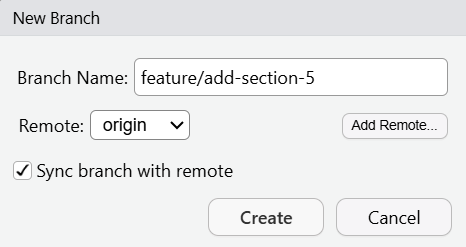
\includegraphics[width=0.2\linewidth]{47_Branch2} \end{flushleft}

\begin{center}\rule{0.5\linewidth}{0.5pt}\end{center}

\subsubsection{5. Best Practices for
Collaboration}\label{best-practices-for-collaboration}

\paragraph{5.1 Do's \& Don'ts (Best Practices for
Collaboration)}\label{dos-donts-best-practices-for-collaboration}

\begin{longtable}[]{@{}
  >{\raggedright\arraybackslash}p{(\linewidth - 2\tabcolsep) * \real{0.5000}}
  >{\raggedright\arraybackslash}p{(\linewidth - 2\tabcolsep) * \real{0.5000}}@{}}
\toprule\noalign{}
\begin{minipage}[b]{\linewidth}\raggedright
✅ Do
\end{minipage} & \begin{minipage}[b]{\linewidth}\raggedright
❌ Don't
\end{minipage} \\
\midrule\noalign{}
\endhead
\bottomrule\noalign{}
\endlastfoot
Pull the latest changes from github before starting the work & Start
editing without pulling an you will be risking everyone project with
that action \\
Commit with understandable, focus and small changes & Make one giant
commit at the end of the day \\
Write a clear commit message for every commit & Use vague messages like
``updates'' or ``changes'' \\
Work on your own branch for each task & Commit directly to `main' \\
Open a Pull Request and have a teammate review before merging & Merge
your own work without a review \\
Talk to the team before making any huge change & Not talking to anyone
before a huge change on the project \\
Use descriptive branch names: `feature/add-graphics', `fix/introduction'
& Use vague branch names like `test', `new', or `edits' \\
\end{longtable}

\paragraph{5.2 Common Errors \& How to resolve
Conflicts:}\label{common-errors-how-to-resolve-conflicts}

\textbf{Error 1: Push Rejected}

\begin{verbatim}
! [rejected] main -> main (fetch first)
error: failed to push some refs to 'https://github.com/...'
\end{verbatim}

\begin{flushleft}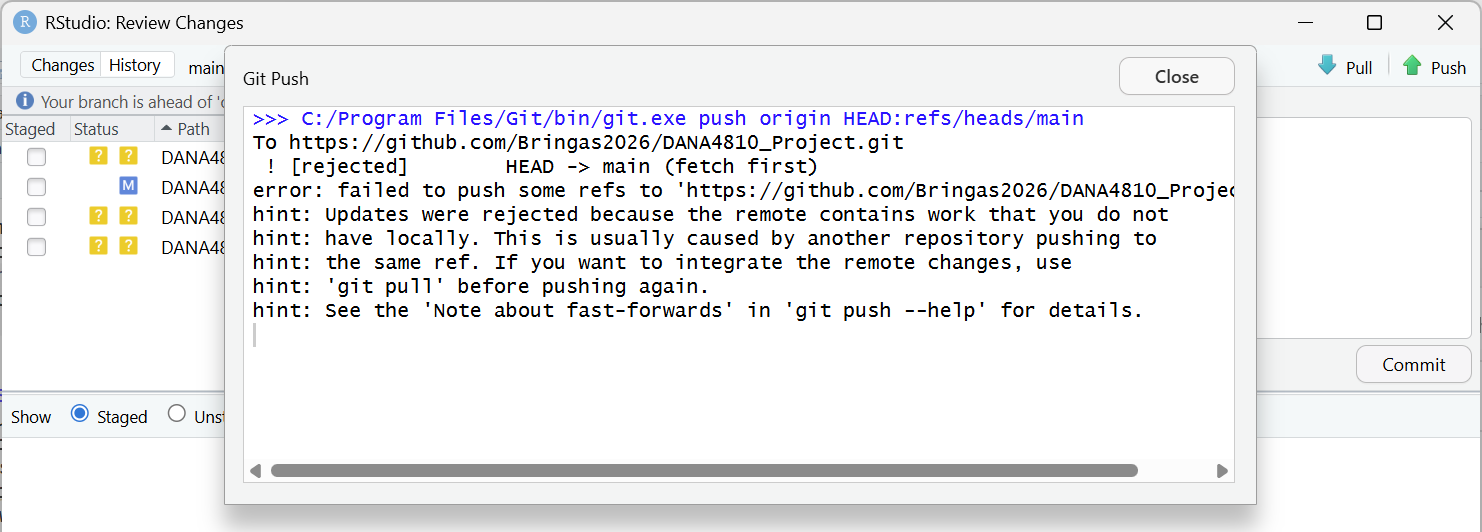
\includegraphics[width=0.8\linewidth]{52_PushRejection} \end{flushleft}

\textbf{What it means:} Someone else pushed changes to GitHub while you
were working. Your local version is now behind the remote version.
\textbf{How to fix it:} Pull first to download the new changes, then
push again. If there are no conflicts, it will work automatically.

\begin{verbatim}
git pull origin main
\end{verbatim}

\textbf{Error 2: Merge Conflict}

\begin{verbatim}
CONFLICT (content): Merge conflict in filename.Rmd
Automatic merge failed; fix conflicts and then commit the result.
\end{verbatim}

\textbf{What it means:} You and a teammate both edited the same lines of
the same file, and Git cannot decide which version to keep. Git will
mark the conflicting section in the file like this:

\begin{verbatim}
<<<<<<< HEAD
Your version of the text here
=======
Your teammate's version of the text here
>>>>>>> 4a01c6e40422fa653d0572728deeef8f3726c90e
\end{verbatim}

\textbf{How to fix it:}

\begin{enumerate}
\def\labelenumi{\arabic{enumi}.}
\tightlist
\item
  Open the file in RStudio. Look for the
  \texttt{\textless{}\textless{}\textless{}\textless{}\textless{}\textless{}\textless{}},
  \texttt{=======}, and
  \texttt{\textgreater{}\textgreater{}\textgreater{}\textgreater{}\textgreater{}\textgreater{}\textgreater{}}
  markers.
\item
  Decide which version to keep (or write a combined version).
\item
  Delete all three marker lines completely.
\item
  Save the file, stage it, and commit:
\end{enumerate}

\begin{verbatim}
git add filename.Rmd
git commit -m "Resolve merge conflict in filename.Rmd"
\end{verbatim}

✅ \textbf{Tip:} The best way to avoid merge conflicts is to Pull at the
start of every session and work on separate files or branches from your
teammates.

\begin{center}\rule{0.5\linewidth}{0.5pt}\end{center}

\subsection{References and Sources}\label{references-and-sources}

\begin{enumerate}
\def\labelenumi{\arabic{enumi}.}
\tightlist
\item
  \textbf{Introduction to GitHub:}
  \url{https://rainsworth.github.io/intro-to-github/06_Collaboration.html}
\item
  \textbf{Earth Data Science:} Github Collaborative Workflow for Team
  Science
  \url{https://earthdatascience.org/courses/intro-to-earth-data-science/git-github/github-collaboration/github-for-collaboration-open-science-workflow/}
\item
  \textbf{GitProtect Blog:} Git Revert File to Previous Commit: How to
  Do It?
  \url{https://gitprotect.io/blog/git-revert-file-to-previous-commit/}
\item
  \textbf{Pro Git Book:} Git Tools - Reset Demystified
  \url{https://git-scm.com/book/en/v2/Git-Tools-Reset-Demystified}
\item
  \textbf{Atlassian Git Tutorials:}
  \url{https://www.atlassian.com/git/tutorials/}
\item
  \textbf{Dangit, Git!?!:} \url{https://dangitgit.com/}
\item
  \textbf{GitHub Docs:} Resolving a merge conflict using the command
  line
  \url{https://docs.github.com/en/pull-requests/collaborating-with-pull-requests/addressing-merge-conflicts/resolving-a-merge-conflict-using-the-command-line}
\end{enumerate}

\begin{center}\rule{0.5\linewidth}{0.5pt}\end{center}

\subsection{Document Update History}\label{document-update-history}

June 15 2026, New Creation

\end{document}
